\documentclass[../../../../main.tex]{subfiles}

\begin{document}

\section*{第1問}

\noindent
[\textbf{解}] $c, d$ の条件は
\begin{align}
ac + bd &= 0 \quad \dots \text{①} \\
c^2 + d^2 &= 1 \quad \dots \text{②}
\end{align}
$ab \neq 0$ から ①より、$d = -\frac{a}{b}c$ だから ②に代入して
\[
\left( 1 + \frac{a^2}{b^2} \right) c^2 = 1
\]
\[
\therefore c = \pm \frac{b}{\sqrt{a^2+b^2}} = \pm \frac{b}{\sqrt{3}}
\]
だから ①に代入して $d = \mp \frac{a}{\sqrt{3}}$（以下複号同順）となるから
\[
(c+d, cd) = \left( \pm \frac{1}{\sqrt{3}}(b-a), \frac{1}{3} \right)
\]
$a, b$ は $\frac{-1 \pm \sqrt{5}}{2}$ をとることから $b-a = \pm \sqrt{5}$ だから
\[
(c+d, cd) = \left( \pm \frac{1}{3}\sqrt{15}, \frac{1}{3} \right)
\]
となり、$c, d$ を 2解に持つ方程式は
\[
x^2 \pm \frac{1}{3}\sqrt{15}x + \frac{1}{3} = 0
\]

\newpage

\section*{第2問}

\noindent
[\textbf{解}] $a > 0$。$f(x) = x[a - (1+a^4)x^2]$ から、$y = f(x)$ と $x$ 軸の交点のうち、$x$ 座標正のもののそれを $c = \sqrt{\frac{a}{1+a^4}}$ である。
\begin{align*}
S_a &= -a^4 \int_0^c x^3 dx + a \int_0^c x dx - \int_0^c x^3 dx \\
\frac{d}{da} S_a &= -a^4 c^3 c' - 4a^3 \int_0^c x^3 dx + \int_0^c x dx + a c c' - c^3 c' \\
&= -(a^4+1)c^3 c' + a c c' + \frac{1}{2}c^2 - a^3 c^4 \quad \dots \text{①}
\end{align*}
又、$a - (a^4+1)c^2 = 0$ だから
\begin{align*}
\frac{dS_a}{da} &= c^2 \left( \frac{1}{2} - \frac{a^4}{1+a^4} \right) \\
&= \frac{-c^2}{2(1+a^4)} (a^2+1)(a^2-1)
\end{align*}
より下表を得る。

\begin{center}
\begin{tabular}{c|ccccc}
$a$ & $0$ & $\dots$ & $1$ & $\dots$ \\ \hline
$S'$ & & $+$ & $0$ & $-$ \\ \hline
$S$ & & $\nearrow$ & & $\searrow$
\end{tabular}
\end{center}

\noindent
よって $S_a$ を最大にする $a$ は $a = 1$。

\newpage

\section*{第3問}

\noindent
[\textbf{解}] $S = \sin x, C = \cos x$ と略記する。漸化式から $k \in \mathbb{Z}_{\ge 0}$ として
\[
f^{4k}(x) = -S, \quad f^{4k+1}(x) = C, \quad f^{4k+2}(x) = -S, \quad f^{4k+3}(x) = -C
\]
である。以下 $P$ の $x$ 座標を $P$ とする。

\begin{enumerate}
    \item[$1^\circ$] $C_1 : y = xS, C_2 : y = C$ の時\\
    $P \sin P = \cos P$ であり、$t_1, t_2$ の接線ベクトルは $\begin{pmatrix} 1 \\ P \cos P + \sin P \end{pmatrix}$, $\begin{pmatrix} 1 \\ -\sin P \end{pmatrix}$ だから
    \[
    \begin{pmatrix} 1 \\ P \cos P + \sin P \end{pmatrix} \cdot \begin{pmatrix} 1 \\ -\sin P \end{pmatrix} = \cos P (\cos P - P \sin P) = 0
    \]
    となり、$t_1$ と $t_2$ は直交する。

    \item[$2^\circ$] $C_1 : y = xC, C_2 : y = -S$ の時\\
    $P \cos P = -\sin P$ であり、接線ベクトルは $\begin{pmatrix} 1 \\ \cos P - P \sin P \end{pmatrix}$, $\begin{pmatrix} 1 \\ -\cos P \end{pmatrix}$ となり、$1^\circ$ と同じく $t_1, t_2$ は直交する。

    \item[$3^\circ$] $C_1 : y = -xS, C_2 : y = -C$ の時\\
    $-P \sin P = -\cos P$ であり、接線ベクトルは $\begin{pmatrix} 1 \\ -P \cos P - \sin P \end{pmatrix}$, $\begin{pmatrix} 1 \\ \sin P \end{pmatrix}$ だから、$1^\circ$ と同じく $t_1, t_2$ は直交する。

    \item[$4^\circ$] $C_1 : y = -xC, C_2 : y = S$ の時\\
    $-P \cos P = \sin P$ であり、接線ベクトルは $\begin{pmatrix} 1 \\ -\cos P + P \sin P \end{pmatrix}$, $\begin{pmatrix} 1 \\ \cos P \end{pmatrix}$ だから、$1^\circ$ と同じく $t_1, t_2$ は直交する。
\end{enumerate}

\noindent
以上から示された。

\newpage

\section*{第4問}

\noindent
[\textbf{解}]
\begin{enumerate}
    \item[(i)] 1回目に出る目の期待値も、2回目に出る目の期待値も $\frac{7}{2}$ だから、
    
    1回目で 3以下なら振り直し、4以上なら振り直さない とすれば良い。

    \item[(ii)] (i)から、3回目をふるかどうかは 2回目が 3以下ならば振り直し、4以上なら振り直さないが良い。この時の 2, 3回目だけの得点の期待値は
    \[
    \frac{1}{6}(4+5+6) + \frac{1}{2} \cdot \frac{7}{2} = \frac{17}{4}
    \]
    だから、1回目に出た目が 4以下ならば振り直し、5以上ならば振り直さなければ良い。
\end{enumerate}

\newpage

\section*{第5問}

\noindent
[\textbf{解}] (1) $a$ 以外の2辺の長さを $x, y$ とする。この時、$x + y = m$ に注意する。

\noindent
$S = \frac{1}{2}(x+y+a) = \frac{1}{2}(m+a)$ としてヘロンの公式から、面積 $T$ として
\begin{align*}
T &= \sqrt{S(S-x)(S-y)(S-a)} \\
&\le \sqrt{S(S-a)} \cdot \frac{(S-x)+(S-y)}{2} \quad (\because S-x, S-y > 0 \text{ から AM-GM}) \\
&= \sqrt{S(S-a)} \cdot \frac{2S-m}{2}
\end{align*}
等号成立は $S-x = S-y \therefore x=y=\frac{m}{2}$ の時。つまり、この時三角形は2等辺三角形である。

\bigskip
\noindent
[\textbf{解2}] $\angle BAC + \angle BDC = \theta$ とする。

\begin{center}
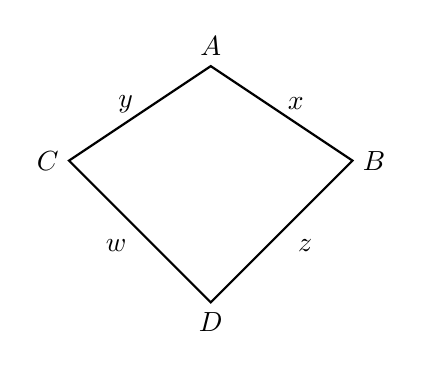
\begin{tikzpicture}[scale=1.2]
    \coordinate (A) at (0, 1.5);
    \coordinate (B) at (1.5, 0.5);
    \coordinate (C) at (-1.5, 0.5);
    \coordinate (D) at (0, -1.0);
    \draw[thick] (A) node[above]{$A$} -- (B) node[right]{$B$} -- (D) node[below]{$D$} -- (C) node[left]{$C$} -- cycle;
    \node at (-0.9, 1.1) {$y$};
    \node at (0.9, 1.1) {$x$};
    \node at (-1.0, -0.4) {$w$};
    \node at (1.0, -0.4) {$z$};
\end{tikzpicture}
\end{center}

\noindent
ブレードシュナイダーの公式から、$S = \frac{1}{2}(x+y+z+w) = \frac{1}{2}m$ として
\begin{align*}
T &= \sqrt{(S-x)(S-y)(S-z)(S-w) - xyzw \cos^2 \frac{\theta}{2}} \\
&\le \sqrt{ \left\{ \frac{(S-x)+(S-y)+(S-z)+(S-w)}{4} \right\}^4 } \quad (\because \text{AM-GM 及び } xyzw \cos^2 \frac{\theta}{2} \ge 0) \\
&= \frac{m^2}{16}
\end{align*}
等号成立は $x=y=z=w$ かつ $\theta=\pi$、つまり $\square ABCD$ が正方形の時。

\bigskip
\noindent
(2) 四角形 $ABCD$ とし、4辺の長さを $x, y, z, w$ とする。この時、$m$ を定数 ($>0$) として
\[
x + y + z + w = m \quad \dots \text{①}
\]
となる。$|BC| = a\ (>0)$, $x+y = k\ (k > a)$ と固定すると、$\triangle ABC$, $\triangle BCD$ は $x=y, z=w$ の時 面積最大である。この面積を $S(k)$ とする。右下図から ($E$ は $BC$ の中点)

\begin{center}
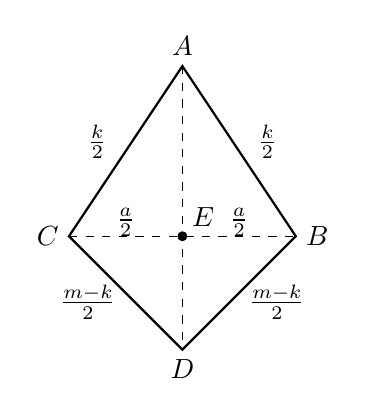
\begin{tikzpicture}[scale=1.2]
    \coordinate (A) at (0, 1.8);
    \coordinate (B) at (1.2, 0);
    \coordinate (C) at (-1.2, 0);
    \coordinate (D) at (0, -1.2);
    \coordinate (E) at (0, 0);
    \draw[thick] (A) node[above]{$A$} -- (B) node[right]{$B$} -- (D) node[below]{$D$} -- (C) node[left]{$C$} -- cycle;
    \draw[dashed] (C) -- (B);
    \draw[dashed] (A) -- (D);
    \fill (E) circle (1.5pt) node[above right]{$E$};
    \node at (-0.6, 0.15) {$\frac{a}{2}$};
    \node at (0.6, 0.15) {$\frac{a}{2}$};
    \node at (-0.9, 1.0) {$\frac{k}{2}$};
    \node at (0.9, 1.0) {$\frac{k}{2}$};
    \node at (-1.0, -0.7) {$\frac{m-k}{2}$};
    \node at (1.0, -0.7) {$\frac{m-k}{2}$};
\end{tikzpicture}
\end{center}

\begin{align*}
S(k) &= \frac{1}{2} a (\overline{AE} + \overline{ED}) \\
&= \frac{1}{2} a \left\{ \sqrt{\left(\frac{k}{2}\right)^2 - \left(\frac{a}{2}\right)^2} + \sqrt{\left(\frac{m-k}{2}\right)^2 - \left(\frac{a}{2}\right)^2} \right\} \\
&\le \frac{1}{2} a \sqrt{(1+1) \left\{ \left(\frac{k}{2}\right)^2 - \left(\frac{a}{2}\right)^2 + \left(\frac{m-k}{2}\right)^2 - \left(\frac{a}{2}\right)^2 \right\}} \quad (\because \text{コーシー・シュワルツ, 等号成立は } k = \frac{1}{2}m) \\
&= \frac{1}{2} a \sqrt{k^2 - mk + \frac{1}{2}m^2 - a^2} \\
&= \frac{1}{2} a \sqrt{\left(k - \frac{1}{2}m\right)^2 + \frac{1}{4}m^2 - a^2} \\
&\le \frac{1}{2} a \sqrt{\frac{1}{4}m^2 - a^2} \quad (\text{等号成立は } k = \frac{1}{2}m)
\end{align*}
だから、$a$ を固定した時、$k = \frac{1}{2}m$ で $S(k)$ は $\max \frac{1}{2} a \sqrt{\frac{1}{4}m^2 - a^2}$ をとる。($\frac{1}{2}m > a$ は満たしている)

\noindent
次に $a$ を動かす。($0 < a < \frac{1}{2}m$)
\begin{align*}
S(k) &= \frac{1}{2} \sqrt{ -a^4 + \frac{1}{4}m^2 a^2 } \\
&= \frac{1}{2} \sqrt{ -\left(a^2 - \frac{1}{8}m^2\right)^2 + \frac{1}{64}m^4 } \\
&\le \frac{1}{16} m^2 \quad (\text{等号成立は } a = \frac{\sqrt{2}}{4}m \text{ のとき})
\end{align*}
したがって $S(k)$ は $a = \frac{\sqrt{2}}{4}m \ (0 < \frac{\sqrt{2}}{4}m < \frac{1}{2}m)$ で $\max$。

\noindent
この時、$x = y = z = w = \frac{1}{4}m, a = \frac{\sqrt{2}}{4}m$ で、たしかに $\square ABCD$ は正方形である。

\noindent
以上から示された。

\newpage

\section*{第6問}

\noindent
[\textbf{解}] (1) (2) (3) に代入して
\begin{equation}
\begin{cases}
-f''(x) \ge f(x) & \dots \text{①} \\
f'(0) = 0 & \dots \text{②} \\
0 \le x \le a \implies f(x) > 0 & \dots \text{③}
\end{cases}
\end{equation}

\begin{enumerate}
    \item[(i)] $0 \le t \le a$ の時、①, ③から
    \[
    -f''(t) > 0
    \]
    $[0, x]\ (0 \le x \le a)$ で積分して
    \[
    f'(0) - f'(x) > 0 \iff 0 > f'(x) \quad (\because \text{②}) \quad \dots \text{④}
    \]
    だから $x = a$ として
    \[
    0 > f'(a) \iff 0 < g(a)
    \]

    \item[(ii)] $a \le y \le a + \frac{f(a)}{-f'(a)}$ で常に $f(y) > 0$ ($f(0) > 0$ と仮定する。③とあわせて
    \[
    \text{「 } 0 \le x \le a - \frac{f(a)}{f'(a)} \text{ で常に } f(x) > 0 \text{ 」} \quad \dots \text{⑤}
    \]
    である。①から、同区間で
    \[
    f''(t) < 0 \quad \therefore f(t) \text{ は単調減少} \quad \dots \text{⑥}
    \]
    となり、④から、$f'(t) \le 0$ つまり $f(t)$ は単調減少である。ここで $f(x)$ には平均値の定理が適用できて、
    \[
    f\left(a - \frac{f(a)}{f'(a)}\right) - f(0) = -\frac{f(a)}{f'(a)} f'(c) \quad \left(a < c < a - \frac{f(c)}{f'(c)}\right)
    \]
    なる $c$ が存在する。変形して
    \[
    f\left(a - \frac{f(a)}{f'(a)}\right) = \frac{f(a)}{f'(a)} \{ f'(a) - f'(c) \} \quad \dots \text{⑦}
    \]
    ここで、⑤, ⑥から
    \[
    f\left(a - \frac{f(a)}{f'(a)}\right) > 0, \quad f(a) > 0, \quad f'(a) < 0
    \]
    だから ⑦より
    \[
    f'(a) - f'(c) < 0 \iff f'(a) < f'(c)
    \]
    しかし、これは ⑥及び $a < c$ に反し矛盾。以上から $a \le y \le a - \frac{f(a)}{f'(a)}$ に $f(y) = 0$ なる $y$ がある。
\end{enumerate}

\end{document}
